\chapter{Equazione Integro-Differenziale del Trasporto Neutronico}

\section{Introduzione}
L'equazione del trasporto neutronico in forma integro-differenziale descrive l'evoluzione temporale e spaziale della densità di neutroni in un mezzo, tenendo conto di processi come la diffusione, l'assorbimento, lo scattering e la fissione. Questo capitolo ne presenta la derivazione sia in approccio Lagrangiano che Euleriano, analizzando le condizioni iniziali, di interfaccia e al contorno, e dimostrandone l’equivalenza con l’equazione di continuità.


\section{Derivazione Lagrangiana}
Consideriamo un fascio di neutroni contenuti in un volume elementare $\mathrm{d}V$ intorno al punto $\mathbf{r}$, con velocità compresa tra $v$ e $v + \mathrm{d}v$ e direzione all’interno dell’angolo solido $\mathrm{d}\Omega$ intorno a $\boldsymbol{\Omega}$. La variazione del numero di neutroni in questo volume durante l’intervallo di tempo $\mathrm{d}t$ è data da:

\begin{equation}
	\delta n\ =\ \left[ n (\mathbf{r} + v \boldsymbol{\Omega} \mathrm{d} t, v \boldsymbol{\Omega}, t + \mathrm{d} t) - n (\mathbf{r}, v \boldsymbol{\Omega}, t) \right] \ \mathrm{d} V\, \mathrm{d} v \,\mathrm{d} \Omega.
\end{equation}

Espandendo in serie di Taylor la densità $n(\mathbf{r} + v\boldsymbol{\Omega}\mathrm{d}t, v\boldsymbol{\Omega}, t + \mathrm{d}t)$ e arrestando lo sviluppo ai termini del primo ordine, otteniamo:

\begin{equation}
	\begin{aligned}
		n (\mathbf{r} + v \boldsymbol{\Omega} \mathrm{d} t, v \boldsymbol{\Omega}, t + \mathrm{d} t)\ &=\ n (\mathbf{r}, v \boldsymbol{\Omega}, t) \\
		&+ \frac{\partial n}{\partial x} \mathrm{d} x + \frac{\partial n}{\partial y} \mathrm{d} y + \frac{\partial n}{\partial z} \mathrm{d} z + \frac{\partial n}{\partial t} \mathrm{d} t + \dots
	\end{aligned}
\end{equation}

Definendo il vettore spostamento:
\begin{equation}
	\left(\mathbf{r} + v \boldsymbol{\Omega} \mathrm{d} t\right)\, -\, \mathbf{r}\ =\ \left(v \Omega_x \mathrm{d} t,\, v \Omega_y \mathrm{d} t,\, v \Omega_z \mathrm{d} t\right)\ =\ (\mathrm{d} x,\, \mathrm{d} y,\, \mathrm{d} z),
\end{equation}
l'equazione precedente può essere riscritta come:

\begin{equation}
	\begin{aligned}
		n (\mathbf{r} + v \boldsymbol{\Omega} \mathrm{d} t, v \boldsymbol{\Omega}, t + \mathrm{d} t) &= n (\mathbf{r}, v \boldsymbol{\Omega}, t) \\
		&+ \left[ \frac{\partial n}{\partial x} v \Omega_x + \frac{\partial n}{\partial y} v \Omega_y + \frac{\partial n}{\partial z} v \Omega_z + \frac{\partial n}{\partial t} \right] \mathrm{d} t + \dots
	\end{aligned}
\end{equation}

I termini all'interno delle parentesi quadre possono essere interpretati come:
\begin{equation}
	\frac{\partial n}{\partial t}\, +\, 
	\textcolor{red}{\left(v \Omega_x \mathbf{i}, v \Omega_y \mathbf{j}, v \Omega_z \mathbf{k}\right)} \cdot \textcolor{blue}{\left(\frac{\partial n}{\partial x} \mathbf{i}, \frac{\partial n}{\partial y} \mathbf{j}, \frac{\partial n}{\partial z} \mathbf{k}\right)}\ =\ \frac{\partial n}{\partial t}\, +\, \textcolor{red}{v \boldsymbol{\Omega}} \cdot \textcolor{blue}{\nabla n}\ \ .
\end{equation}

Da ciò, la variazione $\delta n$ assume la forma:
\begin{equation}
	\delta n\ =\ \left[ \frac{\partial n}{\partial t}\, +\, v \boldsymbol{\Omega} \cdot \nabla n \right]\ \mathrm{d} V \mathrm{d} v \mathrm{d} \Omega \mathrm{d} t.
\end{equation}


\subsection{Contributi alla variazione $\delta n$}
La variazione $\delta n$ è dovuta a diversi contributi, tra cui:
\begin{itemize}[nosep, leftmargin=*]
	\item \textbf{Sorgenti esterne:} $S(\mathbf{r}, v\boldsymbol{\Omega}, t) \cdot \mathrm{d}V  \mathrm{d}v  \mathrm{d}\Omega  \mathrm{d}t$;
	\item \textbf{Rimozione per collisione:} $-\Sigma_t(\mathbf{r}, v)\, v\, n(\mathbf{r}, v\boldsymbol{\Omega}, t) \cdot \mathrm{d}V  \mathrm{d}v  \mathrm{d}\Omega  \mathrm{d}t$;
	\item \textbf{Sorgenti per scattering:}
	\begin{equation}
		\int_{0}^{\infty} \mathrm{d}v' \int_{4\pi} \Sigma_s(\mathbf{r},\, v'\boldsymbol{\Omega}' \rightarrow v\boldsymbol{\Omega})\, v'\, n(\mathbf{r},\, v'\boldsymbol{\Omega}',\, t) \cdot \mathrm{d}\Omega'  \mathrm{d}V  \mathrm{d}v  \mathrm{d}\Omega  \mathrm{d}t;
	\end{equation}
	\item \textbf{Sorgenti per fissione:}
	\begin{equation}
		\chi(v) \int_{0}^{\infty} \mathrm{d}v' \int_{4\pi} \nu \Sigma_f(\mathbf{r}, v') v' n(\mathbf{r}, v'\boldsymbol{\Omega}', t) \cdot \mathrm{d}\Omega' \cdot \mathrm{d}V \cdot \mathrm{d}v \cdot \frac{\mathrm{d}\Omega}{4\pi} \cdot \mathrm{d}t.
	\end{equation}
\end{itemize}

I neutroni di fissione sono assunti essere prodotti isotropicamente, pertanto la frazione emessa all'interno dell'angolo solido $\mathrm{d}\Omega$ è $\frac{\mathrm{d}\Omega}{4\pi}$. Inoltre, si noti che:
\begin{equation}
	\int_{4\pi} \nu \Sigma_f(\mathbf{r}, v') v' n(\mathbf{r}, v'\boldsymbol{\Omega}', t) \cdot \mathrm{d}\Omega' = \nu \Sigma_f(\mathbf{r}, v') \phi(\mathbf{r}, v', t),
\end{equation}
dove $\phi(\mathbf{r}, v', t)$ è il flusso scalare.


\subsection{Forma integro-differenziale dell'equazione del trasporto neutronico}
Combinando i risultati precedenti ed eliminando i differenziali comuni, si ottiene l'equazione integro-differenziale del trasporto neutronico:
\begin{equation}
	\begin{aligned}
		\frac{\partial}{\partial t} n(\mathbf{r}, v\boldsymbol{\Omega}, t) &\,+\, v\boldsymbol{\Omega} \cdot \nabla n(\mathbf{r}, v\boldsymbol{\Omega}, t)\, +\, \Sigma_t(\mathbf{r}, v) v n(\mathbf{r}, v\boldsymbol{\Omega}, t)\ =\\
		&\int_0^\infty \mathrm{d}v' \int_{4\pi}\, \Sigma_s(\mathbf{r},\, v'\boldsymbol{\Omega}' \rightarrow v\boldsymbol{\Omega})\, v'\, n(\mathbf{r}, v'\boldsymbol{\Omega}', t)\, \mathrm{d}\Omega' \\
		&+\, \frac{\chi(v)}{4\pi}\, \int_0^\infty \mathrm{d}v' \,\int_{4\pi} \nu\, \Sigma_f(\mathbf{r}, v')\, v'\, n(\mathbf{r}, v'\boldsymbol{\Omega}', t)\, \mathrm{d}\Omega' \,+\, S(\mathbf{r}, v\boldsymbol{\Omega}, t).
	\end{aligned}
\end{equation}


%%
%
%
\section{Derivazione Euleriana}
L'equazione può essere derivata anche con un approccio Euleriano. Consideriamo un dominio convesso di volume $V$ e scriviamo il bilancio dei neutroni con direzione all'interno dell'angolo solido $\mathrm{d}\Omega$ intorno a $\boldsymbol{\Omega}$ e velocità tra $v$ e $v + \mathrm{d}v$:

\begin{equation}
	\frac{\partial}{\partial t}\, \int_{V}\, n(\mathbf{r}, v \boldsymbol{\Omega}, t) \, \mathrm{d}V \, \mathrm{d}v \, \mathrm{d}\Omega\ =\ \text{(neutron gains)} - \text{(neutron losses)}.
\end{equation}

Se $V$ non dipende dal tempo $t$, l’equazione diventa:
\begin{equation}
	\int_{V}\, \frac{\partial}{\partial t}\, n(\mathbf{r}, v \boldsymbol{\Omega}, t) \, \mathrm{d}V \, \mathrm{d}v \, \mathrm{d}\Omega = \text{(neutron gains)} - \text{(neutron losses)}.
\end{equation}


\subsection{Termini di guadagno}
I termini di guadagno includono:
\begin{itemize}[nosep, leftmargin=*]
	\item \textbf{Sorgenti indipendenti:}
	\begin{equation}
		\int_{V} S(\mathbf{r}, v\boldsymbol{\Omega}, t) \, \mathrm{d}V \, \mathrm{d}v \, \mathrm{d}\Omega\ \ ;
	\end{equation}
	\item \textbf{Sorgenti per scattering:}
	\begin{equation}
		\int_{V} \mathrm{d}V \int_{0}^{\infty} \mathrm{d}v' \int_{4\pi}\ \Sigma_s(\mathbf{r}, v'\boldsymbol{\Omega}' \rightarrow v\boldsymbol{\Omega})\, v'\, n(\mathbf{r}, v'\boldsymbol{\Omega}', t)\ \mathrm{d}\Omega' \, \mathrm{d}v \, \mathrm{d}\Omega\ \ ;
	\end{equation}
	\item \textbf{Sorgenti per fissione:}
	\begin{equation}
		\int_{V} \mathrm{d}V \int_{0}^{\infty} \mathrm{d}v' \int_{4\pi}\ \nu\, \Sigma_f(\mathbf{r}, v')\, v'\, n(\mathbf{r}, v'\boldsymbol{\Omega}', t) \, \mathrm{d}\Omega' \, \chi(v) \, \mathrm{d}v \, \frac{\mathrm{d}\Omega}{4\pi}\ \ .
	\end{equation}
	Si assume che i neutroni di fissione siano prodotti isotropicamente.
\end{itemize}

%
%
\subsection{Termini di perdita}
I termini di perdita includono:
\begin{itemize}[nosep, leftmargin=*]
	\item \textbf{Perdite per collisione:}
	\begin{equation}
		\int_{V} \Sigma_t(\mathbf{r}, v)\, v\, n(\mathbf{r}, v \boldsymbol{\Omega}, t) \ \mathrm{d}V \, \mathrm{d}v \, \mathrm{d}\Omega\ \ ;
	\end{equation}
	\item \textbf{Perdite per fuoriuscita attraverso la superficie di $V$:}
	\begin{equation}
		\int_{S}\ \mathbf{J}(\mathbf{r}, v\boldsymbol{\Omega}, t) \cdot \mathbf{u} \ \mathrm{d}S \, \mathrm{d}v \, \mathrm{d}\Omega\ =\ \int_{V} \nabla \cdot \mathbf{J}(\mathbf{r}, v\boldsymbol{\Omega}, t) \ \mathrm{d}V \, \mathrm{d}v \, \mathrm{d}\Omega,
	\end{equation}
	dove $\mathbf{J}(\mathbf{r}, v\boldsymbol{\Omega}, t) = n(\mathbf{r}, v\boldsymbol{\Omega}, t)\, v\boldsymbol{\Omega}$ è la corrente neutronica. Sviluppando, si ottiene:
	\begin{equation}
		\int_{V} v\boldsymbol{\Omega} \cdot \nabla n(\mathbf{r}, v\boldsymbol{\Omega}, t) \, \mathrm{d}V \, \mathrm{d}v \, \mathrm{d}\Omega.
	\end{equation}
\end{itemize}


\subsection{Equazione finale}
Raccogliendo tutti i termini, si perviene alla stessa equazione integro-differenziale derivata con l'approccio Lagrangiano.

\section{Condizioni iniziali, di interfaccia e al contorno}

\subsection{Condizione iniziale}
La condizione iniziale è classica: si assume nota la distribuzione del flusso angolare (o della densità) al tempo $t = 0$:
\begin{equation}
	\phi(\mathbf{r}, E, \boldsymbol{\Omega}, 0) = \phi_0(\mathbf{r}, E, \boldsymbol{\Omega}).
\end{equation}

\subsection{Condizione di interfaccia}
Attraverso un’interfaccia, il numero di neutroni che viaggiano in una certa direzione si conserva, pertanto la condizione è la continuità del flusso angolare (o della densità). Questa condizione non vale nel caso in cui l’interfaccia rappresenti una sorgente superficiale o una cortina assorbente.

\subsection{Condizioni al contorno}
\subsubsection{Superficie libera (interfaccia con il vuoto)}

\begin{multicols}{2}
Per un dominio convesso $V$ completamente circondato dal vuoto, non possono esserci neutroni che entrano in $V$ attraverso il suo contorno $\delta V$. I neutroni che escono dal dominio non possono rientrare. La condizione al contorno è quindi:
\begin{equation}
	\phi(\mathbf{r}, E, \boldsymbol{\Omega}, t) = 0; \quad \forall \boldsymbol{\Omega}: \boldsymbol{\Omega} \cdot \mathbf{u} < 0, \mathbf{r} \in \delta V,
\end{equation}
dove $\mathbf{u}$ è la normale uscente al contorno in $\mathbf{r}$.

\begin{figure}[H]
	\centering
	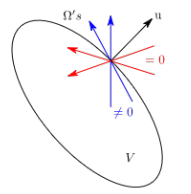
\includegraphics[width=0.6\linewidth]{img/integrodifferential1.png}
\end{figure}

\end{multicols}


\subsubsection{Flusso entrante imposto}
Se il flusso entrante è noto, la condizione al contorno diventa:
\begin{equation}
	\phi(\mathbf{r}, E, \boldsymbol{\Omega}, t) = \psi(\mathbf{r}, E, \boldsymbol{\Omega}, t); \quad \forall \boldsymbol{\Omega}: \boldsymbol{\Omega} \cdot \mathbf{u} < 0, \mathbf{r} \in \delta V.
\end{equation}

\subsubsection{Condizione di riflessione speculare}

\begin{multicols}{2}
Con probabilità $\alpha$, che può dipendere dall’energia, i neutroni che attraversano il contorno $\delta V$ del dominio $V$ vengono riflessi specularmente. La condizione è:
\begin{equation}
	\phi (\mathbf{r}, E, \boldsymbol{\Omega}, t) = \alpha (E) \phi (\mathbf{r}, E, \boldsymbol{\Omega}', t); \quad \forall \boldsymbol{\Omega}: \boldsymbol{\Omega} \cdot \mathbf{u} < 0, \mathbf{r} \in \delta V,
\end{equation}
dove:
\begin{equation}
	\boldsymbol{\Omega} \cdot \mathbf{u} = - \boldsymbol{\Omega}' \cdot \mathbf{u},
\end{equation}
e
\begin{equation}
	\left(\boldsymbol{\Omega} \times \boldsymbol{\Omega}'\right) \cdot \mathbf{u} = 0.
\end{equation}
La condizione appena presentata assicura la planarità dei tre vettori $\boldsymbol{\Omega}$, $\boldsymbol{\Omega}'$ e $\mathbf{u}$. Il fattore $\alpha(E)$ è detto coefficiente di albedo. Il caso $\alpha(E) = 1$ corrisponde a una riflessione pura.

\begin{figure}[H]
	\centering
	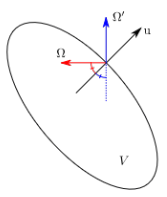
\includegraphics[width=0.4\linewidth]{img/integrodifferential2.png}
\end{figure}
\end{multicols}



\subsubsection{Riflessione diffusa o condizione di contorno "bianca"}
Tutti i neutroni che attraversano il contorno di $V$ in $\mathbf{r}$ rientrano all’interno di $V$ con una distribuzione angolare isotropica sulle direzioni entranti. Quindi:
\begin{equation}
	J_u^- (\mathbf{r}, E, t) = J_u^+ (\mathbf{r}, E, t); \quad \mathbf{r} \in \delta V \quad (\text{entrante} = \text{uscente}),
\end{equation}
dove:
\begin{equation}
	\phi (\mathbf{r}, E, \boldsymbol{\Omega}, t) = C (\mathbf{r}, E, t); \quad \forall \boldsymbol{\Omega}: \boldsymbol{\Omega} \cdot \mathbf{u} < 0, \mathbf{r} \in \delta V.
\end{equation}
\begin{multicols}{2}
La corrente entrante $J_u^-$ è definita come:
\begin{equation}
	\begin{aligned}
		J_u^- (\mathbf{r}, E, t) &= \left| \mathbf{u} \cdot \int_{\boldsymbol{\Omega} \cdot \mathbf{u} < 0} \phi (\mathbf{r}, E, \boldsymbol{\Omega}, t) \boldsymbol{\Omega} \, \mathrm{d}\Omega \right| \\
		&= \int_{\boldsymbol{\Omega} \cdot \mathbf{u} < 0} \phi (\mathbf{r}, E, \boldsymbol{\Omega}, t) | \boldsymbol{\Omega} \cdot \mathbf{u} | \, \mathrm{d}\Omega \\
		&= \int_{\boldsymbol{\Omega} \cdot \mathbf{u} < 0} C (\mathbf{r}, E, t) | \boldsymbol{\Omega} \cdot \mathbf{u} | \, \mathrm{d}\Omega.
	\end{aligned}
\end{equation}
\begin{figure}[H]
	\centering
	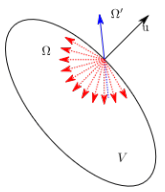
\includegraphics[width=0.4\linewidth]{img/integrodifferential3.png}
\end{figure}
\end{multicols}

Sapendo che:
\begin{equation}
	| \boldsymbol{\Omega} \cdot \mathbf{u} | = | \cos \theta | = | \mu |,
\end{equation}
e
\begin{equation}
	\mathrm{d}\Omega = \sin \theta \, \mathrm{d}\theta \, \mathrm{d}\varphi = - \mathrm{d}\varphi \, \mathrm{d}\mu,
\end{equation}
si ottiene:
\begin{equation}
	\begin{aligned}
		J_u^- (\mathbf{r}, E, t) &= \int_{0}^{2\pi} \mathrm{d}\varphi \int_{-1}^{0} C (\mathbf{r}, E, t) (-\mu) \, \mathrm{d}\mu \\
		&= 2\pi \left( - \frac{1}{2} \mu^2 \Bigg|_{-1}^{0} \right) C (\mathbf{r}, E, t) \\
		&= \pi C (\mathbf{r}, E, t).
	\end{aligned}
\end{equation}

Grazie alla condizione \eqref{cond:entrante=uscente}, si ricava:
\begin{equation}
	C (\mathbf{r}, E, t) = \frac{1}{\pi} J_u^+ (\mathbf{r}, E, t); \quad \mathbf{r} \in \delta V.
\end{equation}

Infine, la condizione al contorno \eqref{cond:isotropica} può essere riscritta come:
\begin{equation}
	\phi (\mathbf{r}, E, \boldsymbol{\Omega}, t) = \frac{1}{\pi} J_u^+ (\mathbf{r}, E, t); \quad \forall \boldsymbol{\Omega}: \boldsymbol{\Omega} \cdot \mathbf{u} < 0, \mathbf{r} \in \delta V,
\end{equation}
dove:
\begin{equation}
	J_u^+ (\mathbf{r}, E, t) = \int_{\boldsymbol{\Omega} \cdot \mathbf{u} > 0} \phi (\mathbf{r}, E, \boldsymbol{\Omega}, t) \boldsymbol{\Omega} \cdot \mathbf{u} \, \mathrm{d}\Omega.
\end{equation}

\subsubsection{Condizione periodica}
Questa condizione è particolarmente adatta per domini che si ripetono regolarmente nello spazio, come la cella di combustibile o l’assieme di combustibile. Il flusso angolare entrante nella posizione $\mathbf{r}$ sul contorno è impostato uguale al flusso angolare uscente dal punto speculare $\mathbf{r} \pm \mathbf{r}_l$ sulla superficie opposta:
\begin{equation}
	\phi (\mathbf{r}, \boldsymbol{\Omega}, E, t) = \phi (\mathbf{r} + \mathbf{r}_l, \boldsymbol{\Omega}, E, t),
\end{equation}
\begin{equation}
	\phi (\mathbf{r}, \boldsymbol{\Omega}, E, t) = \phi (\mathbf{r} - \mathbf{r}_l, \boldsymbol{\Omega}, E, t).
\end{equation}

\begin{figure}[H]
	\centering
	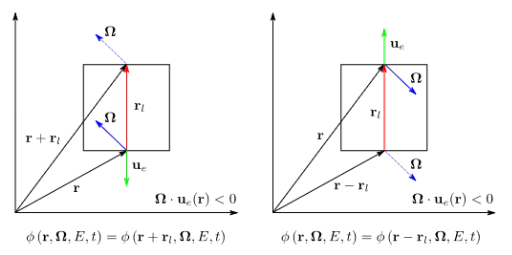
\includegraphics[width=0.7\linewidth]{img/integrodifferential4.png}
\end{figure}


%
%
%
\section{Equivalenza tra equazione del trasporto neutronico e equazione di continuità}

L’equazione del trasporto scritta in termini del flusso neutronico angolare può essere dimostrata equivalente all’equazione di continuità in termini del flusso neutronico scalare. Partendo dall'equazione del trasporto, riscritta in termini del flusso angolare dipendente dall’energia:
\begin{equation}
	\begin{aligned}
		\frac{1}{v} \frac{\partial}{\partial t} \phi (\mathbf{r}, E, \boldsymbol{\Omega}, t)\ &+\ \boldsymbol{\Omega} \cdot \nabla \phi (\mathbf{r}, E, \boldsymbol{\Omega}, t)\ +\ \Sigma_t (\mathbf{r}, E) \phi (\mathbf{r}, E, \boldsymbol{\Omega}, t) =\\
		&\int_0^\infty \mathrm{d}E' \int_{4\pi} \Sigma_s (\mathbf{r}, E' \rightarrow E, \boldsymbol{\Omega}' \rightarrow \boldsymbol{\Omega}) \phi (\mathbf{r}, E', \boldsymbol{\Omega}', t) \, \mathrm{d}\Omega' \\
		&+ \frac{\chi(E)}{4\pi} \int_0^\infty \mathrm{d}E' \int_{4\pi} \nu \Sigma_f (\mathbf{r}, E') \phi (\mathbf{r}, E', \boldsymbol{\Omega}', t) \, \mathrm{d}\Omega' \\
		&+ S (\mathbf{r}, E, \boldsymbol{\Omega}, t).
	\end{aligned}
\end{equation}

Integrare entrambi i membri su tutto l’angolo solido $\mathrm{d}\Omega$:

\subsubsection{Termini del lato sinistro}
\begin{itemize}[nosep, leftmargin=*]
	\item Primo termine:
	\begin{equation}
		\frac{1}{v} \frac{\partial}{\partial t} \int_{4\pi} \phi (\mathbf{r}, E, \boldsymbol{\Omega}, t) \, \mathrm{d}\Omega = \frac{1}{v} \frac{\partial}{\partial t} \phi (\mathbf{r}, E, t).
	\end{equation}
	
	\item Secondo termine:
	\begin{equation}
		\boldsymbol{\Omega} \cdot \nabla \phi = \nabla \cdot (\boldsymbol{\Omega} \phi),
	\end{equation}
	quindi:
	\begin{equation}
		\int_{4\pi} \boldsymbol{\Omega} \cdot \nabla \phi (\mathbf{r}, E, \boldsymbol{\Omega}, t) \, \mathrm{d}\Omega = \nabla \cdot \int_{4\pi} \boldsymbol{\Omega} \phi (\mathbf{r}, E, \boldsymbol{\Omega}, t) \, \mathrm{d}\Omega = \nabla \cdot \mathbf{J} (\mathbf{r}, E, t).
	\end{equation}
	
	\item Terzo termine:
	\begin{equation}
		\int_{4\pi} \Sigma_t(\mathbf{r}, E) \phi(\mathbf{r}, E, \boldsymbol{\Omega}, t) \, \mathrm{d}\Omega = \Sigma_t(\mathbf{r}, E) \phi(\mathbf{r}, E, t).
	\end{equation}
\end{itemize}

\subsubsection{Termini del lato destro}
\begin{itemize}[nosep, leftmargin=*]
	\item Integrale di scattering: integrando le direzioni uscenti $\mathbf{\Omega}$ elimina anche le dipendenze dalle direzioni entranti $\mathbf{\Omega'}$, così la sezione d'urto differenziale di scattering dipende da $\mathbf{\Omega\cdot\Omega'}$
	\begin{equation}
		\begin{aligned}
			\int_{4\pi} &\left[ \int_0^\infty \mathrm{d}E' \int_{4\pi} \Sigma_s(\mathbf{r}, E' \to E, \boldsymbol{\Omega}' \to \boldsymbol{\Omega}) \phi(\mathbf{r}, E', \boldsymbol{\Omega}', t) \, \mathrm{d}\Omega' \right] \, \mathrm{d}\Omega \\
			&= \int_0^\infty \mathrm{d}E' \int_{4\pi} \Sigma_s(\mathbf{r}, E' \to E) \phi(\mathbf{r}, E', t) \, \mathrm{d}E'.
		\end{aligned}
	\end{equation}
	
	\item Sorgente di fissione:
	\begin{equation}
		\begin{aligned}
			\int_{4\pi} \left[ \frac{\chi(E)}{4\pi} \int_0^\infty \nu \Sigma_f (\mathbf{r}, E') \phi (\mathbf{r}, E', t) \, \mathrm{d}E' \right] \, \mathrm{d}\Omega &= \chi(E) \int_0^\infty \nu \Sigma_f (\mathbf{r}, E') \phi (\mathbf{r}, E', t) \, \mathrm{d}E'.
		\end{aligned}
	\end{equation}
	
	\item Sorgente generale:
	\begin{equation}
		\int_{4\pi} S (\mathbf{r}, E, \boldsymbol{\Omega}, t) \, \mathrm{d}\Omega = S (\mathbf{r}, E, t).
	\end{equation}
\end{itemize}

%%
%
%
\subsection{Equazione di continuità}
Sommando tutti i contributi, l’equazione \eqref{eq:trasporto_energia} diventa:
\begin{equation}
	\begin{aligned}
		\frac{1}{v} \frac{\partial}{\partial t} \phi(\mathbf{r}, E, t) + \nabla \cdot \mathbf{J}(\mathbf{r}, E, t) + \Sigma_t(\mathbf{r}, E) \phi(\mathbf{r}, E, t) &= \int_0^\infty \Sigma_s(\mathbf{r}, E' \to E) \phi(\mathbf{r}, E', t) \, \mathrm{d}E' \\
		&+ \chi(E) \int_0^\infty \nu \Sigma_f(\mathbf{r}, E') \phi(\mathbf{r}, E', t) \, \mathrm{d}E' \\
		&+ S(\mathbf{r}, E, t).
	\end{aligned}
\end{equation}
Questa è la ben nota \textbf{equazione di continuità neutronica}.


\section{Approssimazioni dello Scattering: Isotropico e Linearmente Anisotropico}

\subsection{Introduzione}
In questa sezione vengono presentate le approssimazioni della sezione d'urto differenziale di scattering per l'equazione del trasporto neutronico in regime stazionario e monocinetico. In particolare, verranno analizzate le espansioni in polinomi di Legendre per lo scattering isotropico, linearmente anisotropico e quadraticamente anisotropico.


\subsection{Espansione della sezione d’urto di scattering}
L'equazione integro-differenziale del trasporto neutronico in \underline{regime stazionario} e \underline{monocinetico} ha la forma:
\begin{equation}
	\boldsymbol{\Omega} \cdot \nabla n (\mathbf{r}, \boldsymbol{\Omega}) + \Sigma_t (\mathbf{r}) n (\mathbf{r}, \boldsymbol{\Omega}) = \int_{4\pi} \Sigma_s (\mathbf{r}, \boldsymbol{\Omega}' \rightarrow \boldsymbol{\Omega}) n (\mathbf{r}, \boldsymbol{\Omega}') \, \mathrm{d}\Omega' + \frac{1}{4\pi} \int_{4\pi} \nu \Sigma_f (\mathbf{r}) n (\mathbf{r}, \boldsymbol{\Omega}') \, \mathrm{d}\Omega' + S (\mathbf{r}, \boldsymbol{\Omega}).
\end{equation}

Come emerso nella teoria del rallentamento dei neutroni, la sezione d’urto differenziale di scattering $\Sigma_s(\mathbf{r}, \boldsymbol{\Omega}' \rightarrow \boldsymbol{\Omega})$ dipende dal coseno dell’angolo di deviazione $\mu_0 = \boldsymbol{\Omega} \cdot \boldsymbol{\Omega}'$, cioè:
\begin{equation}
	\Sigma_s (\mathbf{r}, \boldsymbol{\Omega}' \rightarrow \boldsymbol{\Omega}) = \Sigma_s (\mathbf{r}, \mu_0) = \Sigma_s (\mathbf{r}, \cos \psi).
\end{equation}

\begin{approfondimento}{Espansione in polinomi di Legendre}
La parte angolare della sezione d'urto differenziale viene solitamente espansa in termini di polinomi di Legendre:

\begin{equation}\label{espansione legendre}
	\Sigma_s (\mathbf{r}, \mu_0) = \sum_{l=0}^{\infty} \frac{2l + 1}{4\pi} \Sigma_{sl} (\mathbf{r}) P_l (\mu_0),
\end{equation}
\begin{multicols}{2}
dove $\mu_0$ è il coseno dell'angolo di deviazione (o angolo di scattering, i.e. $\mu_0 =\cos \psi$).
\begin{figure}[H]
	\centering
	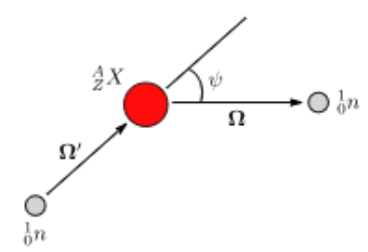
\includegraphics[width=0.4\linewidth]{img/legendre1.png}
\end{figure}
\end{multicols}
I polinomi di Legendre sono definiti ricorsivamente come:
\begin{equation}
	\begin{aligned}
		P_0 (\mu_0) &= 1, \\
		P_1 (\mu_0) &= \mu_0, \\
		P_{l+1} (\mu_0) &= \frac{2l + 1}{l + 1} \mu_0 P_l (\mu_0) - \frac{l}{l + 1} P_{l-1} (\mu_0).
	\end{aligned}
\end{equation}

\begin{figure}[H]
	\centering
	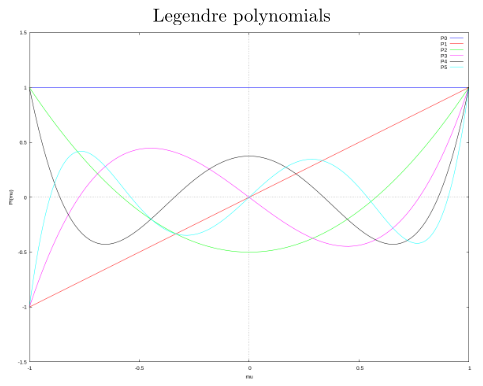
\includegraphics[width=0.5\linewidth]{img/legendre2.png}
\end{figure}

I polinomi di Legendre sono funzioni ortogonali nell’intervallo $[-1, 1]$:
\begin{equation}
	\int_{-1}^{1} P_k(\mu_0) P_l(\mu_0) \, \mathrm{d}\mu_0 = \frac{2}{2l + 1} \delta_{lk},
\end{equation}
e
\begin{equation}
	\int_{-1}^{1} P_l(\mu_0) \, \mathrm{d}\mu_0 = \frac{2}{2l + 1} \delta_{l0} =
	\begin{cases}
		2 & \text{se } l = 0, \\
		0 & \text{se } l \neq 0.
	\end{cases}
\end{equation}


\end{approfondimento}

Dall'espansione vista con Legendre, integrando su tutto l’angolo solido, si ottiene:
\begin{equation}
	\begin{aligned}
		\Sigma_s(\mathbf{r}) &= \int_{4\pi} \Sigma_s(\mathbf{r}, \boldsymbol{\Omega}' \rightarrow \boldsymbol{\Omega}) \, \mathrm{d}\Omega \\
		&= \int_{4\pi} \sum_{l=0}^{\infty} \frac{2l + 1}{4\pi} \Sigma_{sl}(\mathbf{r}) P_l(\mu_0) \, \mathrm{d}\Omega \\
		&= \sum_{l=0}^{\infty} \frac{2l + 1}{4\pi} \Sigma_{sl}(\mathbf{r}) \int_{0}^{2\pi} \mathrm{d}\varphi \int_{-1}^{1} P_l(\mu_0) \, \mathrm{d}\mu_0 \\
		&= \Sigma_{s0}(\mathbf{r}).
	\end{aligned}
\end{equation}


\subsection{Approssimazione di scattering isotropico}

Nell'approssimazione di scattering isotropico, l’espansione della sezione d’urto differenziale viene troncata al primo termine:
\begin{equation}
	\Sigma_s (\mathbf{r}, \mu_0)\ =\ \frac{1}{4\pi} \Sigma_{s0} (\mathbf{r}) P_0 (\mu_0) = \frac{1}{4\pi} \Sigma_{s0} (\mathbf{r}).
\end{equation}

Poiché $\Sigma_{s0}(\mathbf{r}) = \Sigma_s(\mathbf{r})$, l’equazione precedente diventa:
\begin{equation}
	\boxed{\ \Sigma_s (\mathbf{r}, \mu_0)\ =\ \frac{\Sigma_s (\mathbf{r})}{4\pi}\ }\ \ .
\end{equation}


\subsection{Approssimazione di scattering linearmente anisotropico}
L'espansione della sezione d'urto differenziale viene ora troncata al secondo termine:
\begin{equation}
	\Sigma_s(\mathbf{r}, \mu_0)\ =\ \frac{1}{4\pi} \Sigma_{s0}(\mathbf{r}) P_0(\mu_0) + \frac{3}{4\pi} \Sigma_{s1}(\mathbf{r}) P_1(\mu_0).
\end{equation}
Sostituendo i polinomi di Legendre:
\begin{equation}
	\Sigma_s(\mathbf{r}, \mu_0)\ =\ \frac{1}{4\pi} \Sigma_{s0}(\mathbf{r}) + \frac{3}{4\pi} \Sigma_{s1}(\mathbf{r}) \mu_0\  .
\end{equation}

Il coefficiente $\Sigma_{s0}(\mathbf{r})$ è lo stesso ottenuto nello scattering isotropico, cioè $\Sigma_{s0}(\mathbf{r}) = \Sigma_s(\mathbf{r})$.


\subsubsection{Determinazione di $\Sigma_{s1}(\mathbf{r})$ e coefficiente medio del coseno dell’angolo di deviazione}
Per determinare $\Sigma_{s1}(\mathbf{r})$, moltiplichiamo entrambi i membri dell’equazione appena ricavata (per lo scattering linearmente anisotropico) per $P_1(\mu_0)$ e integriamo su tutto l’angolo solido:
\begin{equation}
	\begin{aligned}
		\int_{4\pi} \Sigma_s(\mathbf{r}, \mu_0) P_1(\mu_0) \, \mathrm{d}\Omega &= \int_{4\pi} \frac{\Sigma_{s0}(\mathbf{r})}{4\pi} P_0(\mu_0) P_1(\mu_0) \, \mathrm{d}\Omega \\
		&\quad + \int_{4\pi} \frac{3}{4\pi} \Sigma_{s1}(\mathbf{r}) P_1(\mu_0) P_1(\mu_0) \, \mathrm{d}\Omega.
	\end{aligned}
\end{equation}

Sviluppando gli integrali:
\begin{equation}
	\begin{aligned}
		2\pi \int_{-1}^{1} \Sigma_s(\mathbf{r}, \mu_0) \mu_0 \, \mathrm{d}\mu_0 &= \frac{\Sigma_{s0}(\mathbf{r})}{2} \int_{-1}^{1} P_0(\mu_0) P_1(\mu_0) \, \mathrm{d}\mu_0 \\
		&\quad + \frac{3}{2} \Sigma_{s1}(\mathbf{r}) \int_{-1}^{1} P_1(\mu_0) P_1(\mu_0) \, \mathrm{d}\mu_0 \\
		&= \Sigma_{s1}(\mathbf{r}),
	\end{aligned}
\end{equation}
dove si è usato il fatto che $\int_{-1}^{1} P_1(\mu_0) P_1(\mu_0) \, \mathrm{d}\mu_0 = \frac{2}{3}$.

Seconda la definizione del coseno medio dell’angolo di deviazione:
\begin{equation}
	\bar{\mu}_0 = \frac{\int_{0}^{2\pi} \mathrm{d}\varphi \int_{-1}^{1} \Sigma_s(\mathbf{r}, \mu_0) \mu_0 \, \mathrm{d}\mu_0}{\int_{0}^{2\pi} \mathrm{d}\varphi \int_{-1}^{1} \Sigma_s(\mathbf{r}, \mu_0) \, \mathrm{d}\mu_0} = \frac{2\pi \int_{-1}^{1} \Sigma_s(\mathbf{r}, \mu_0) \mu_0 \, \mathrm{d}\mu_0}{\Sigma_s(\mathbf{r})},
\end{equation}
da cui:
\begin{equation}
	2\pi \int_{-1}^{1} \Sigma_s(\mathbf{r}, \mu_0) \mu_0 \, \mathrm{d}\mu_0 = \bar{\mu}_0 \Sigma_s(\mathbf{r}).
\end{equation}

Quindi, dall’equazione \eqref{eq:sigma_s1_integrale}:
\begin{equation}
	\Sigma_{s1}(\mathbf{r}) = \bar{\mu}_0 \Sigma_s(\mathbf{r}).
\end{equation}

\subsubsection{Forma finale dello scattering linearmente anisotropico}
L'espansione della sezione d'urto differenziale diventa:
\begin{equation}
	\Sigma_s (\mathbf{r}, \mu_0) = \frac{1}{4\pi} \Sigma_{s0} (\mathbf{r}) P_0 (\mu_0) + \frac{3}{4\pi} \Sigma_{s1} (\mathbf{r}) P_1 (\mu_0),
\end{equation}
che, sostituendo i coefficienti, assume la forma:
\begin{equation}
	\boxed{\ \Sigma_s (\mathbf{r}, \mu_0) = \frac{\Sigma_s (\mathbf{r})}{4\pi} (1 + 3 \bar{\mu}_0 \mu_0)\ }\ \ .
\end{equation}


\section{Approssimazione di scattering quadraticamente anisotropico}
Nell'approssimazione quadratica dell'anisotropia di scattering, l’espansione diventa:
\begin{equation}
	\Sigma_s(\mathbf{r}, \mu_0)\ =\ \frac{1}{4\pi} \Sigma_{s0}(\mathbf{r}) P_0(\mu_0)\, +\, \frac{3}{4\pi} \Sigma_{s1}(\mathbf{r}) P_1(\mu_0)\, +\, \frac{5}{4\pi} \Sigma_{s2}(\mathbf{r}) P_2(\mu_0)\ \ .
\end{equation}

L'unico momento da determinare è $\Sigma_{s2}(\mathbf{r})$. Moltiplicando entrambi i membri per $P_2(\mu_0)$ e integrando su tutto l'angolo solido, i primi due termini a destra si annullano, quindi:
\begin{equation}
	\begin{aligned}
		2\pi \int_{-1}^{1} \Sigma_s(\mathbf{r}, \mu_0) P_2(\mu_0) \, \mathrm{d}\mu_0\ &=\ \frac{5}{2} \Sigma_{s2}(\mathbf{r}) \int_{-1}^{1} P_2(\mu_0) P_2(\mu_0) \, \mathrm{d}\mu_0 \\
		&=\ \Sigma_{s2}(\mathbf{r}),
	\end{aligned}
\end{equation}
dove si è usato $\int_{-1}^{1} P_2(\mu_0) P_2(\mu_0) \, \mathrm{d}\mu_0 = \frac{2}{5}$.


\subsubsection{Determinazione di $\Sigma_{s2}(\mathbf{r})$}
Sostituendo l'espressione di $P_2(\mu_0) = \frac{1}{2} (3\mu_0^2 - 1)$, si ottiene:
\begin{equation}
	\begin{aligned}
		\Sigma_{s2}(\mathbf{r}) &= 2\pi \int_{-1}^{1} \Sigma_s(\mathbf{r}, \mu_0) \frac{1}{2} (3\mu_0^2 - 1) \, \mathrm{d}\mu_0 \\
		&= \frac{3}{2} \left(2\pi \int_{-1}^{1} \Sigma_s(\mathbf{r}, \mu_0) \mu_0^2 \, \mathrm{d}\mu_0\right) - \frac{1}{2} \left(2\pi \int_{-1}^{1} \Sigma_s(\mathbf{r}, \mu_0) \, \mathrm{d}\mu_0\right) \\
		&= \frac{3}{2} \left(2\pi \int_{-1}^{1} \Sigma_s(\mathbf{r}, \mu_0) \mu_0^2 \, \mathrm{d}\mu_0\right) - \frac{1}{2} \Sigma_s(\mathbf{r}).
	\end{aligned}
\end{equation}

Dalla definizione del coseno quadratico medio dell'angolo di scattering:
\begin{equation}
	\overline{\mu_0^2}\ =\ \frac{\int_{0}^{2\pi} \mathrm{d}\varphi \int_{-1}^{1} \Sigma_s(\mathbf{r}, \mu_0) \mu_0^2 \, \mathrm{d}\mu_0}{2\pi \int_{-1}^{1} \Sigma_s(\mathbf{r}, \mu_0) \, \mathrm{d}\mu_0}\ =\ \frac{2\pi \int_{-1}^{1} \Sigma_s(\mathbf{r}, \mu_0) \mu_0^2 \, \mathrm{d}\mu_0}{\Sigma_s(\mathbf{r})},
\end{equation}
si ha:
\begin{equation}
	2\pi \int_{-1}^{1} \Sigma_s(\mathbf{r}, \mu_0) \mu_0^2 \, \mathrm{d}\mu_0\ =\ \overline{\mu_0^2}\, \Sigma_s(\mathbf{r})\ \ .
\end{equation}

Quindi, l'equazione per $\Sigma_{s2}(\mathbf{r})$ diventa:
\begin{equation}
	\Sigma_{s2}(\mathbf{r})\ =\ \frac{3}{2} \overline{\mu_0^2} \Sigma_s(\mathbf{r})\, -\, \frac{1}{2} \Sigma_s(\mathbf{r})\ =\ \frac{1}{2} \Sigma_s(\mathbf{r}) \left(3 \overline{\mu_0^2} - 1\right)\ \ .
\end{equation}


\subsubsection{Forma finale dello scattering quadraticamente anisotropico}
Infine, l'equazione per lo scattering quadraticamente anisotropico può essere riscritta come:
\begin{equation}
	\Sigma_s(\mathbf{r}, \mu_0) = \frac{\Sigma_s(\mathbf{r})}{4\pi} \left[ 1 + 3 \bar{\mu}_0 \mu_0 + \frac{5}{2} \left(3 \overline{\mu_0^2} - 1\right) \left(\frac{3\mu_0^2 - 1}{2}\right) \right].
\end{equation}